%%%%%%%%%%%%%%%%%%%%%%%%%%%%%%%%%%%%%%%%%%%%%%%%%%%%%%%%%%%%%%%%%%%%%%%%
% Plantilla TFG/TFM
% Escuela Politécnica Superior de la Universidad de Alicante
% Realizado por: Jose Manuel Requena Plens
% Contacto: info@jmrplens.com / Telegram:@jmrplens
%%%%%%%%%%%%%%%%%%%%%%%%%%%%%%%%%%%%%%%%%%%%%%%%%%%%%%%%%%%%%%%%%%%%%%%%

\chapter{Antecedentes Metodológicos y Tecnológicos}
\label{Antecedentes Metodológicos y Tecnológicos}
En el siguiente capítulo, se presentan los métodos y tecnologías que son necesarias
conocer para el planteamiento apropiado del método usado para la reconstrucción del cuerpo humano 3D, que constituye el núcleo del presente trabajo y que se detalla en el capitulo X.
Primero, se detallará el método de adquisición 3D que tiene PIFu[\cite{pifu}]. 
\section{Introducción}

El proyecto se ha iniciado usando el método desarrollado en PIFu [\cite{pifu}] 

Como se ha dicho antes en el capítulo \ref{sec:Introducción} PIFu [\cite{pifu}] alinea de manera local las características individuales a nivel de píxel con el contexto global de todo el objeto, esto lo hace de una manera totalmente convolucional, esto ayuda a que no requiere un alto uso de memoria como en otro tipo de representaciones, esto es relevante para la reconstrucción 3D de personas con ropa cuya forma puede ser muy deformable, detallada y con una topología complicada.

En concreto se entrena un encoder (codificador) que aprenda sobre vectores de características para cada píxel que existe en la imagen teniendo en cuenta el contexto global relativo a su posición, con este vector y una profundidad en el eje z especificada a lo largo del rayo de cámara saliente del píxel, aprende a partir de una función implícita que puede clasificar si un punto 3D correspondiente a esta profundidad z está dentro o fuera de la superficie.

\begin{figure}[H]
	\centering
	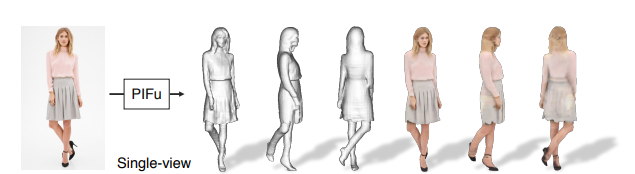
\includegraphics[scale=0.7]{imagenes/antecedentes1.png}
	\caption{Pixel-aligned Implicit function (PIFu) [\cite{pifu}].}
	\label{fig:figura7}
\end{figure}

\subsection{Pixel-aligned Implicit function, PIFu}

Dada una vista, el objetivo es reconstruir la geometría 3D y textura de un humano vestido mientras se intenta preservar los detalles presentes en la imagen. Para realizar esto de una manera eficiente se propone el uso de una función implícita, dado que esta define una superficie como un level-set(conjunto de nivel,  ) de una función. Esta forma de representar las superficies es eficiente porque la superficie embebida no necesita ser explícitamente almacenada en la memoria. La propuesta que realizan consiste en un codificador $g$ de imágenes totalmente convolucional y una función $f$ continua e implícita representada por una red MLP (multi-layer perceptrons), donde la superficie esta definida como un conjunto de nivel de:
\begin{equation}
	f(F(x), z(X)) = s : s \in \mathbb{R}
\end{equation}
donde para un punto 3D $X$, $x = \pi(X)$ es su proyección 2D, $z(X)$ es el valor de profundidad en el espacio de coordenadas de la cámara, $F(x) = g(I(x))$ es la característica de la imagen en $x$. Se obtiene la función de alineamiento $F(X)$ usando un muestreo bilineal, porque la proyección 2D de $X$ se define en un espacio continuo en lugar de uno discreto (es decir, píxel).

\begin{figure}[H]
	\centering
	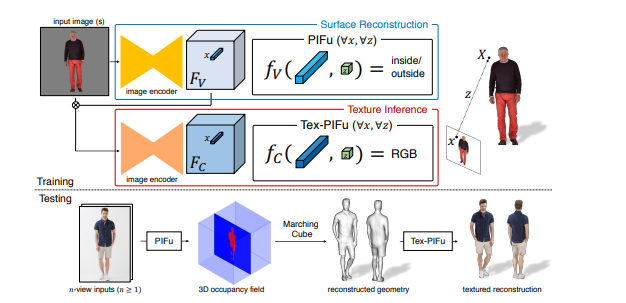
\includegraphics[scale=0.7]{imagenes/antecedentes2.png}
	\caption{Pipeline usada en (PIFu) [\cite{pifu}]. Dada una imagen, PIFu predice la probabilidad continua interior/exterior de un cuerpo humano vestido. Tex-PIFu infiere un valor RGB dados los puntos 3D de la superficie con  con topología arbitraria}
	\label{fig:figura8}
\end{figure}

 Para la reconstrucción de la superficie, se representa como un conjunto de nivel de 0,5 dentro de un campo continuo 3D:
 \begin{equation}
 	f_{v}^{*} = \begin{cases}
 				1\text{,}  & \text{X esta dentro de la superficie de la malla}\\
 				0\text{,}  & \text{resto de casos}\\
 			\end{cases}
 \end{equation}

Se entrena PIFu $f_{v}$ minimizando la media del mean squared error (MSE)

\begin{equation}
	\mathcal{L}_{V} = \frac{1}{n} 
	\sum_{i=1}^{n} | f_{v} (F_{V}(x_{i}) z(X_{i})) - f_{v}^{*}(X_{i}) |^{2}
\end{equation}
 


